\documentclass[sn-mathphys-num]{sn-jnl}% Math and Physical Sciences Numbered Reference Style 

\usepackage{graphicx}%
\usepackage{multirow}%
\usepackage{amsmath,amssymb,amsfonts}%
\usepackage{amsthm}%
\usepackage{mathrsfs}%
\usepackage[title]{appendix}%
\usepackage{xcolor}%
\usepackage{textcomp}%
\usepackage{manyfoot}%
\usepackage{booktabs}%
\usepackage{algorithm}%
\usepackage{algorithmicx}%
\usepackage{algpseudocode}%
\usepackage{listings}%
\usepackage{orcidlink}
\usepackage{xcolor}


\newtheorem{theorem}{Theorem}%
\newtheorem{example}{Example}%
\newtheorem{remark}{Remark}%
\newtheorem{definition}{Definition}%

\raggedbottom

\begin{document}

\title[Clima Craft]{Clima Craft}

\author{Ashwin Vazhappilly\,\orcidlink{0009-0009-6725-4367} (Matriculation number: 5575882)}


\affil{\orgdiv{Informatik}, \orgname{Albert-Ludwigs-Universität Freiburg}, \orgaddress{\city{Freiburg}, \postcode{79117}, \state{Baden-Württemberg}, \country{Germany}}}

\maketitle

\section{Introduction}\label{sec1}

Weather information is a critical resource for daily planning, agriculture, travel, and numerous other sectors. Traditional weather applications provide basic forecast data; however, there is a growing need for more interactive and detailed weather reporting tools. To address this, we introduce ClimaCraft, a lightweight and innovative Python GTK application designed to fetch, display, and graphically represent weather information from OpenWeatherMap.org in a user-friendly manner. ClimaCraft leverages a combination of real-time data fetching, graphical data representation through GNUPlot, and a unique feature that generates narrative weather reports in LaTeX PDF format, making it a versatile tool for both personal and professional use.

The development of ClimaCraft was motivated by the desire to improve accessibility to weather information through enhanced visualization and narrative reporting. By integrating with OpenWeatherMap.org, ClimaCraft provides up-to-date weather forecasts, including temperature, wind, and precipitation details. The application's graphical representations offer users an intuitive understanding of weather patterns, while the LaTeX PDF report generation feature allows for the creation of detailed, printable weather narratives.

This paper presents an overview of ClimaCraft, including its features, installation process, and usage instructions. We detail the application's technological framework, which utilizes Python 3 for its core functionality, GNUPlot for graphical representation, and a suite of LaTeX packages for document generation. Through this work, we aim to contribute to the advancement of weather information dissemination, offering a tool that not only presents data but does so in a manner that is both informative and engaging for the user. 

\section{System Architecture and Design}\label{sec2}

Adopting a modular architectural design, especially for complex software applications like ClimaCraft, offers significant advantages over traditional, monolithic or tightly coupled architectures. This approach divides the application into distinct modules—each with specific functionalities such as the Presentation Layer, Business Logic Layer, Data Access Layer, and Reporting Module—enabling a more streamlined, efficient, and flexible development process. In ClimaCraft, components like the UI and CSS codes, API calls, data management, and report generation operate semi-independently yet remain interconnected, enhancing development, maintenance, scalability, and usability.

The integration of Python 3 and GTK3 (GIMP Toolkit 3) further elevates ClimaCraft by leveraging a lightweight, yet powerful framework for creating graphical user interfaces. Python 3’s clear syntax and powerful libraries, combined with GTK3’s capabilities for developing attractive, responsive UIs, make ClimaCraft not only functional but also accessible and engaging for users. This combination supports the modular architecture's goal of maintainability and scalability by allowing for rapid development and iteration of user interface components without sacrificing performance or user experience.

Maintainability and scalability are central to ClimaCraft’s design philosophy, facilitated by its modular structure. This approach allows developers to update, debug, or enhance specific application parts without impacting the whole, significantly reducing error introduction and maintaining system stability. It inherently supports scalability, enabling seamless integration of new features as distinct modules. The architecture also promotes efficiency and reusability by allowing for parallel development processes and code reuse across different application areas or in future projects, ensuring consistency and quality throughout. Furthermore, the decoupling of modules increases reliability and simplifies testing and debugging, enabling independent module verification for quality and performance.

\section{Implementation}\label{sec3}

\subsection{API Calls}\label{sec3.1}

In ClimaCraft, the implementation of API calls for fetching real-time and forecasted weather data is central to its functionality. Through specialized functions like \texttt{get\_simplified\_weather\_info}, \texttt{get\_wind\_and\_pressure\_info}, and \texttt{get\_additional\_weather\_info}, the application adeptly gathers and presents current weather conditions, wind specifics, and additional meteorological details. This structured approach not only enhances modularity and maintainability but also ensures that users receive tailored weather information efficiently.

To address the need for forecasted weather data, ClimaCraft employs a strategic method to minimize API calls and optimize data storage. By fetching up to seven days of forecast data and incorporating a logic to prevent redundant data storage—updating the stored data only when discrepancies arise—the application significantly improves performance and efficiency. This careful balance between data retrieval frequency and storage optimization underscores ClimaCraft's innovative design in managing forecast information effectively.

Moreover, ClimaCraft's ability to compare current weather conditions with forecasted data provides users with valuable insights into weather trends. This feature not only enriches the user experience by offering a detailed analysis of weather patterns but also exemplifies the application's commitment to delivering comprehensive and actionable weather information. Through these strategies, ClimaCraft sets itself apart as an advanced tool for weather data visualization and analysis, enhancing decision-making and planning based on accurate weather forecasts.

\subsection{GUI Development with Python, GTK3, and Glade}\label{sec3.2}

In developing ClimaCraft, significant emphasis was placed on creating a user-friendly and efficient Graphical User Interface (GUI), achieved through the integration of Python 3 and GTK3 with Glade. This approach combines the versatility and clarity of Python with GTK3's capabilities for crafting responsive and aesthetically pleasing interfaces, further enhanced by Glade's visual design tools and CSS support for styling. This combination underpins the modular architecture of ClimaCraft, aligning with its core principles of maintainability, scalability, and user engagement.

Glade, a RAD tool that enables developers to design a GUI in a WYSIWYG environment, emerges as a critical asset in this development framework. It allows for the separation of interface design from code logic, enabling designers and developers to collaborate more effectively without interfering with each other's work. This separation is particularly beneficial in a modular architecture like ClimaCraft's, where it contributes to the system's overall maintainability and scalability. Designers can update the GUI without altering the underlying codebase, and developers can modify the backend without affecting the interface layout. Additionally, Glade's support for CSS styling enhances the ability to create visually engaging and consistent user interfaces without extensive manual coding, thereby increasing development efficiency.

Moreover, the implementation of threading technology for background data processing and the incorporation of interactive elements, such as the refresh and download buttons, exemplify the application's responsiveness and user-centered design. Threading ensures that the GUI remains responsive, even when performing intensive tasks like fetching weather data or rendering graphs using GNUPlot. This approach minimizes latency and improves the user experience by allowing the application to perform background operations without freezing the interface.

\subsection{GNUplot}\label{sec3.3}

In the realm of ClimaCraft, the innovative use of GNUplot for visualizing weather data stands as a cornerstone of its functionality and appeal. This visualization transcends mere graphical representation to offer a sophisticated interpretation of complex weather patterns, achieved through meticulously crafted Python scripts. These scripts are integral to ClimaCraft's architecture, transforming raw weather data into insightful graphical narratives that significantly enhance the application's value to its users.

The first script, dedicated to weather comparison, embarks on the crucial task of parsing weather data from CSV files containing observed and predicted metrics. It dynamically generates GNUplot commands to construct a bar graph, illustrating the disparities or congruences between actual weather outcomes and forecasts. This process begins with extracting relevant weather parameters from the CSV file, which are then plotted as histograms to facilitate an intuitive visual comparison. The script meticulously sets the graph's aesthetic and functional parameters, including size, data representation style, and axes labels and ranges. Notably, 'set style' and 'plot' commands fine-tune the histograms' visual appearance and accurately map the actual versus predicted data onto the graph. This attention to detail ensures the resultant graph is not only informative but also easy to interpret, with the x-axis representing weather parameters and the y-axis their values, thus clearly depicting forecast accuracy.

The script focusing on wind speed and gust direction operates by first extracting unique month names from a CSV file, ensuring the graph provides a temporal context that is both accurate and meaningful. The script's core lies in its construction of a GNUplot command sequence that specifies the graph's dimensions, output format, and data properties, achieving a detailed visualization of wind patterns over time. The y-axes, dedicated to wind speed, gust, and direction, allow for a comprehensive analysis within a single graphical output, effectively conveying the nuanced behavior of wind over the selected period.

Similarly, the script for the temperature versus precipitation plot generates a dual-axis graph that distinguishes between temperature and precipitation on separate y-axes, enhancing interpretability and allowing viewers to draw correlations between these crucial weather parameters. The script configures GNUplot with custom line styles and colors for different data types, ensuring the visual output is both informative and aesthetically pleasing.

Behind the scenes, the execution of these scripts involves creating a temporary GNUplot script file, which is run to generate the graph and then deleted to maintain a clean working environment. This process underscores ClimaCraft's sophisticated use of technology to present complex weather data in an accessible format. By leveraging advanced plotting tools like GNUplot, ClimaCraft not only advances weather information visualization but also demonstrates the effectiveness of combining programming expertise with graphical tools to tackle intricate data visualization challenges.

\subsection{Latex}\label{sec3.4}

ClimaCraft introduces an innovative feature in weather data visualization and reporting by incorporating LaTeX, an advanced typesetting system, to generate detailed weather reports. This functionality is realized through a Python script that transforms weather data fetched via API into a narrative and graphical report, articulated in a LaTeX document. The script meticulously processes temperature conditions, wind speed, and other meteorological data, embedding them within a narrative framework that dynamically adjusts based on specific weather conditions. For instance, conditional loops within the script generate narrative segments tailored to the current temperature, offering insights that are both informative and engaging. This approach not only enhances the readability of the report but also contextualizes the data in a manner that resonates with the reader's daily experience.

The LaTeX report generated by ClimaCraft is structured to emulate the comprehensive coverage found in newspaper weather reports, incorporating various sections that detail temperature, wind conditions, and comparative analyses of actual versus predicted weather data. The inclusion of graphical data visualizations, generated through integrated GNUplot scripts, further enriches the report, offering readers a visual representation of weather trends and patterns. This integration of textual and graphical information is facilitated by LaTeX's robust package ecosystem and TeX Live, enabling the creation of documents that are both aesthetically pleasing and highly informative. The report culminates in a PDF document, compiled directly within the application's environment, and made readily available for download. This process underscores ClimaCraft's commitment to leveraging cutting-edge technologies to enhance user engagement and understanding of weather information.

The technical architecture behind this feature exemplifies a seamless fusion of data retrieval, processing, and presentation layers within ClimaCraft's modular design. By employing Python for data processing and narrative generation, and LaTeX for document compilation, the application demonstrates an effective use of programming and typesetting languages to create a user-centric product. The automated compilation of LaTeX into a PDF document, executed through command-line instructions within the Python environment, reflects a sophisticated approach to software development that prioritizes efficiency, reliability, and user accessibility. This innovative use of LaTeX in ClimaCraft not only sets a new standard for weather reporting applications but also contributes to the broader field of data visualization and automated report generation, offering insights and methodologies that may benefit future research and development in similar domains.

\subsection{Dockerized Visualization \& Scripting}\label{sec3.5}

ClimaCraft integrates weather data visualization and narrative report generation within a Dockerized environment, addressing the complexities of deploying a GTK-based GUI application across varied computing environments. This containerization strategy ensures consistent and reliable execution by encapsulating the application, its dependencies, and the runtime environment, thus overcoming platform-specific constraints.

\subsubsection{Dockerization Strategy}\label{sec3.5.1}
The deployment strategy begins with a Python 3.10 base image, optimizing for the latest Python features and security enhancements. The Dockerfile configures the working directory to \texttt{/app} and installs essential dependencies, including a comprehensive suite of LaTeX packages for report generation, GTK 3 and GObject introspection libraries for GUI rendering, and Gnuplot for graphical data visualization. This setup ensures that all necessary tools for compiling LaTeX documents and executing the GUI are available within the containerized environment, facilitating effortless generation and access to detailed weather reports.

\subsubsection{GUI Support and PDF Generation}\label{sec3.5.2}
GUI support in the containerized ClimaCraft application is achieved through the \texttt{run.sh} script, which sets up X11 forwarding to enable the GUI's display on the host's system. This script manages the Docker container's lifecycle from initiation to termination and handles the retrieval of generated PDF reports, demonstrating seamless integration between the containerized application and the host system. It leverages Docker's volume and file copy capabilities to extract the \texttt{weather\_report.pdf} to the host's Downloads directory, thus ensuring that users can easily access the generated reports. This meticulous approach to GUI support and PDF generation via Docker and X11 forwarding highlights ClimaCraft's dedication to providing an accessible, efficient, and user-friendly experience, serving as a model for the deployment of GUI-based applications in the modern era of containerization.


\subsection{Github Actions}\label{sec3.6}
To ensure the robustness and cross-platform compatibility of ClimaCraft's Dockerized environment, the project incorporates a GitHub CI/CD workflow named "Cross-Platform Docker Build." This workflow is triggered on every push to the main branch or pull request against it, leveraging GitHub Actions to automate the Docker build process across different environments, specifically focusing on Linux via ubuntu-latest runner.

The workflow begins with checking out the latest code from the repository. It then optimizes the build process by caching Python dependencies, significantly reducing build times for subsequent runs. The caching mechanism uses a unique key based on the operating system and the hash of the requirements.txt file, ensuring that dependencies are re-used when unchanged.

Following dependency caching, the workflow proceeds to build the Docker image on a Linux environment. This step is critical for verifying that the Docker container, along with all its dependencies and the application itself, is built successfully and is ready to be deployed or tested further. This automated process not only streamlines the development workflow but also ensures that the Docker image is consistently tested across the intended deployment platform, maintaining the reliability and stability of ClimaCraft's application delivery.

\section{Features and Screenshots}\label{sec4}

ClimaCraft is a Python GTK application designed to provide users with comprehensive and interactive weather information. Leveraging data from OpenWeatherMap.org, it presents weather details in both graphical formats and narrative reports. Here's an overview of its key features:
\begin{itemize}
    \item Fetches real-time and forecasted weather data from OpenWeatherMap.org.
    \item Displays weather information, including temperature, wind, and precipitation details.
    \item Offers a graphical representation of weather forecasts using GNUPlot for intuitive visualization.
    \item Automatically generates narrative weather reports in LaTeX PDF format for detailed analysis.
    \item Features a modular architecture design for enhanced maintainability and scalability.
    \item Provides a user-friendly GUI developed with Python 3, GTK3, and Glade, supporting CSS for styling.
    \item Manages efficient API calls to optimize data fetching and storage.
    \item Includes comprehensive weather data visualization scripts for comparing actual vs. forecasted weather, wind patterns, and temperature vs. precipitation.
    \item Supports Dockerization for easy installation and deployment, ensuring a consistent environment setup.
\end{itemize}

\begin{figure}[htbp]
    \centering
    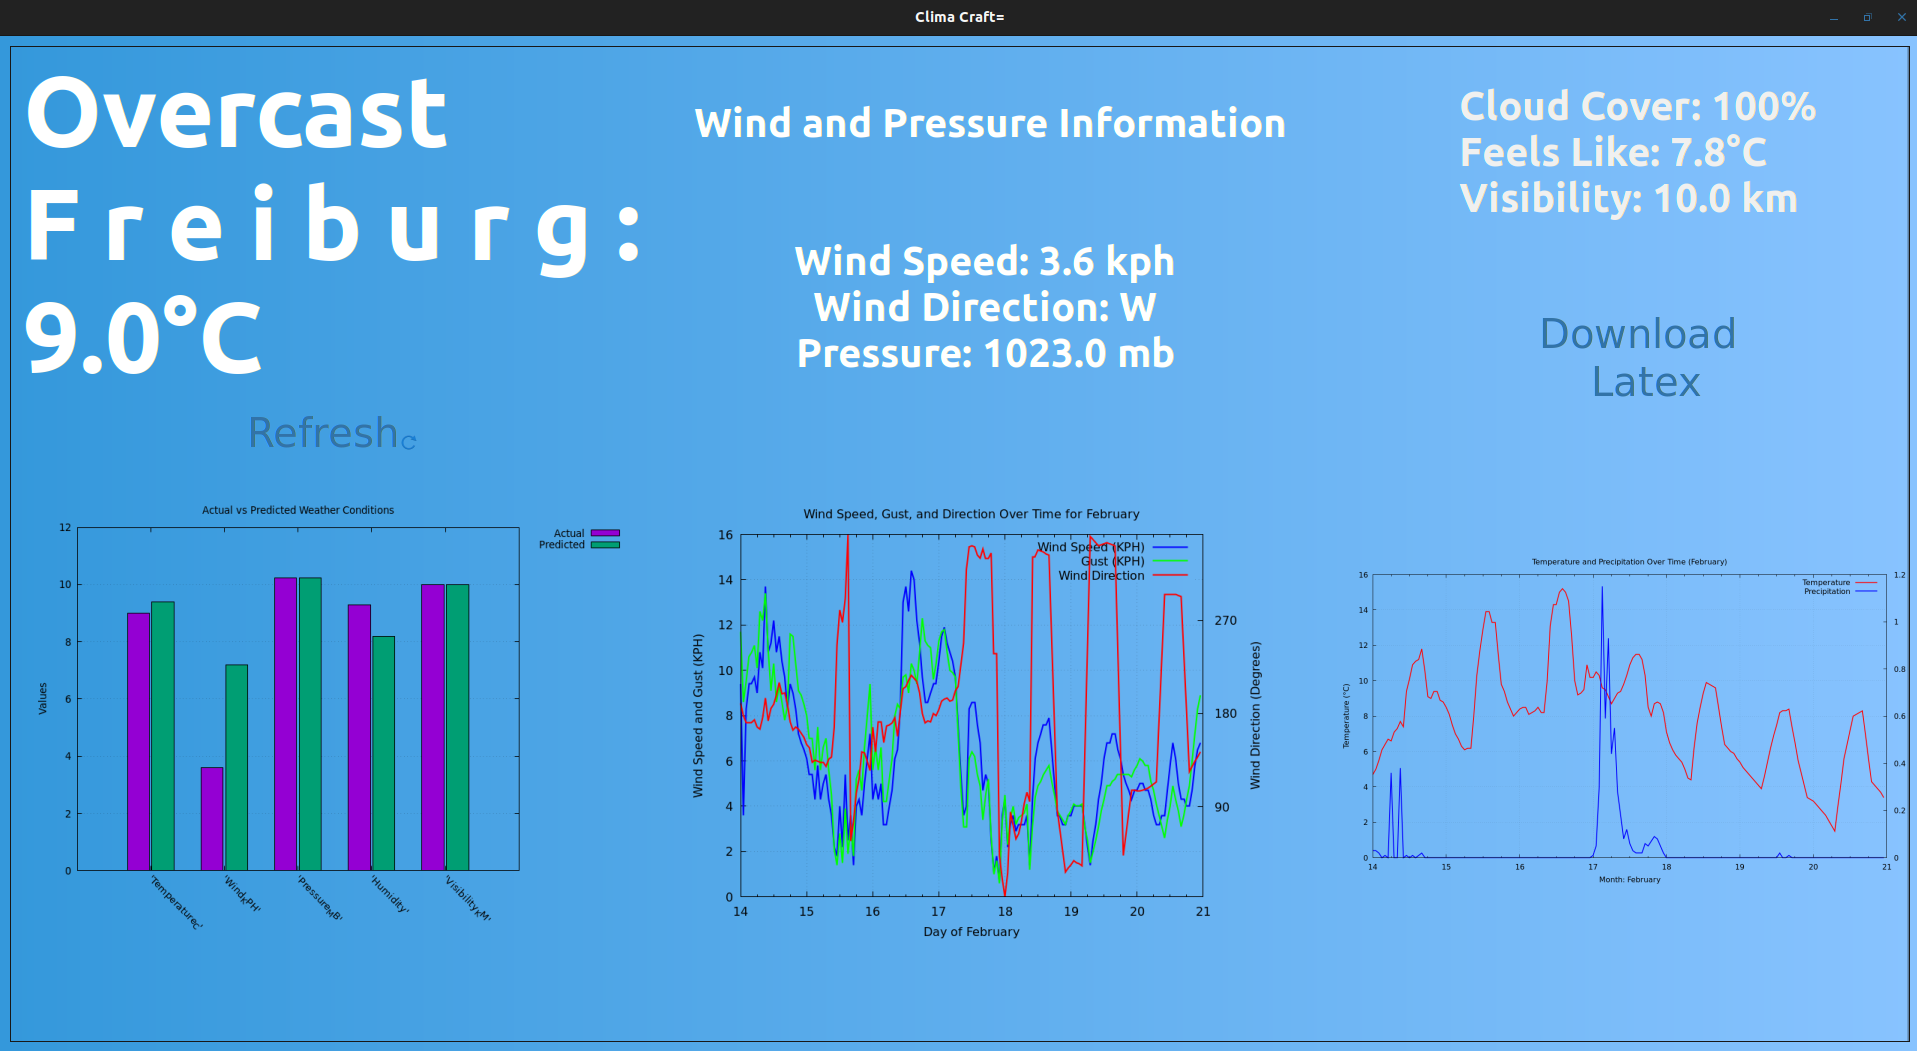
\includegraphics[width=0.70\textwidth]{Mainwindow.png}
    % Manually center the caption
    \parbox{\textwidth}{\centering Fig 1 The main window of ClimaCraft.}
    \label{fig:mainwindow}
\end{figure}

\begin{figure}[htbp]
    \centering
    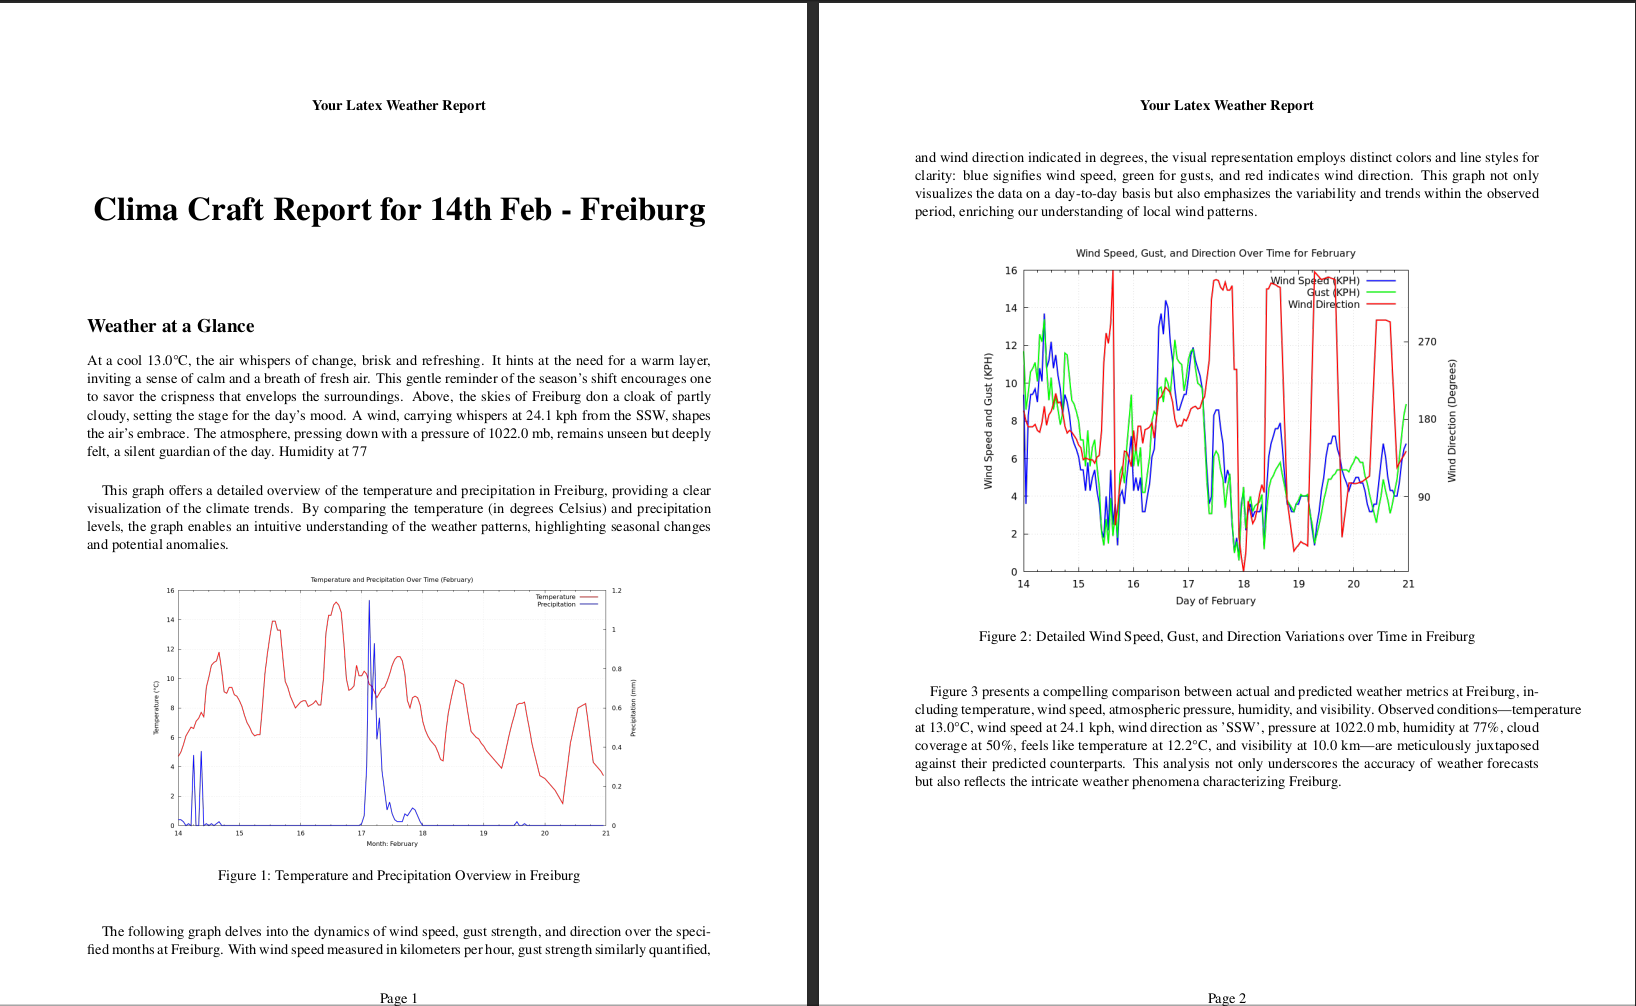
\includegraphics[width=0.70\textwidth]{Latexreport.png}
    % Manually center the caption
    \parbox{\textwidth}{\centering Fig 2 A LaTeX report generated by ClimaCraft.}
    \label{fig:latexreport}
\end{figure}

\clearpage

\section{Conclusion and Future Work}\label{sec5}

\subsection{Conclusion}\label{sec5.1}
ClimaCraft has demonstrated remarkable effectiveness as a Python GTK application, providing users with a comprehensive and interactive weather information platform. By leveraging data from OpenWeatherMap.org, the application not only fetches real-time and forecasted weather data but also presents this information through intuitive graphical formats and detailed narrative reports. The inclusion of various graphs, such as comparisons of current weather conditions, wind and gust patterns, as well as temperature and precipitation correlations, stands out as a testament to ClimaCraft's analytical capabilities. Additionally, its user-friendly GUI and the generation of LaTeX reports for download further enhance its utility, offering users a materialistic view of weather data and the convenience of documenting these insights.

The modular architecture and the careful consideration given to the application's design and development reflect a commitment to maintainability, scalability, and user engagement. These attributes not only underscore ClimaCraft's current success but also lay a solid foundation for future enhancements.

\subsection{Future Work}\label{sec5.2}
As ClimaCraft embarks on its journey towards expanding its utility and enhancing user experience, several ambitious developments are on the horizon. The initiative to open-source the project is a pivotal step that will invite collaboration and innovation from the global developer community. This strategic move is expected to accelerate feature development, facilitate bug fixes, and enable the integration of new data sources, significantly enriching the application's weather reporting capabilities.

A notable feature in development is the dynamic adaptation of the application's background color to reflect current weather conditions. This endeavor has already seen preliminary efforts, but challenges related to CSS integration, particularly when running inside Docker, where CSS does not render as expected, have been encountered. Recognizing the importance of this immersive feature, dedicated effort will be directed towards overcoming these technical obstacles to ensure that the application's visual experience aligns closely with real-world weather conditions.

Furthermore, ClimaCraft plans to extend its data offerings to include more detailed weather analytics, such as air quality indices and long-term climate trends. These enhancements will not only equip users with more comprehensive insights into weather patterns but also bolster support for research and educational projects.

Another critical area of development is the distribution of ClimaCraft. Efforts to deploy the application on official software stores for various platforms, particularly aiming for an exclusive release on the Ubuntu operating system, are underway. This will involve navigating the specific requirements and processes of various Linux app stores, such as Snapcraft for Snap packages, the Debian Package Manager for Debian-based distributions, and possibly Flatpak for a wide range of Linux environments. Simplifying the installation process through one-click downloads and installations is expected to significantly broaden the application's user base and foster a more engaged community.

In making ClimaCraft open-source, the project aspires to become one of the official app for the community, encouraging contributions that can enhance its functionality and user interface. Additionally, the integration of machine learning for weather prediction marks an exciting avenue of future work. Leveraging machine learning algorithms to analyze historical weather data and predict future conditions aligns with the project's commitment to leveraging cutting-edge technology to enhance weather forecasting. This initiative not only represents an intersection of technology and meteorology but also serves as a practical application of academic studies in real-world scenarios.

In conclusion, ClimaCraft's evolution from a highly effective weather application to a platform with advanced features and broader accessibility exemplifies the essence of continuous improvement and innovation. The project's forward momentum, driven by collaborative development, technological advancements, and a focus on user experience, positions ClimaCraft to become an indispensable resource for weather enthusiasts, researchers, and the general public. Through open-source collaboration and the incorporation of predictive analytics, ClimaCraft is set to redefine the standards of weather applications.

\begin{thebibliography}{99}

\bibitem{ieee2018consumer}
"Development of a Weather Application in Android and iOS Operating Systems," \emph{2018 IEEE International Conference on Consumer Electronics-Taiwan (ICCE-TW)}, 2018, https://ieeexplore.ieee.org/document/8448971/references\#references.

\bibitem{pythonGtkTutorial}
"Python GTK+ 3 Tutorial," https://python-gtk-3-tutorial.readthedocs.io.

\bibitem{weatherApi}
"Weather API," https://www.weatherapi.com/.

\bibitem{ieee2020weatherApp}
"Development of a Weather Application in Android and iOS Operating Systems," \emph{IEEE}, 2020, https://ieeexplore.ieee.org/document/9042141.

\bibitem{ieee2011gui}
"Interactive evolution of graphical user interface with GTK toolkit," \emph{IEEE}, 2011, https://ieeexplore.ieee.org/document/5999457.

\bibitem{gladeWiki}
"Glade (Programmierwerkzeug)," \emph{Wikipedia}, https://de.wikipedia.org/wiki/Glade

\bibitem{mediumModularArch}
"On Modular Architectures," \emph{Medium}, https://medium.com/on-software-architecture/on-modular-architectures-53ec61f88ff4.

\bibitem{gnuplotInfo}
"Gnuplot," http://www.gnuplot.info/.

\bibitem{texLive}
"TeX Live," https://www.tug.org/texlive/.

\bibitem{gtkOrg}
"GTK," https://www.gtk.org/.

\bibitem{githubCiCd}
"CI/CD with GitHub Actions," https://resources.github.com/ci-cd/.

\bibitem{chatGpt}
"OpenAI ChatGPT," \emph{OpenAI }, https://chat.openai.com/.

\end{thebibliography}

\vspace{108pt}

\begin{table}[htbp]
\centering
\resizebox{\textwidth}{!}{
\begin{tabular}{|l|p{0.7\textwidth}|}
\hline
\textbf{Topics} & \textbf{Details} \\
\hline
Linux & App developed primarily for Linux; development conducted on Linux using GTK; Linux native app. \\
\hline
Text Editor & Used PyCharm and Glade for the design part; added various GTK extensions. \\
\hline
Git & Implemented a CI/CD action in GitHub to check the Docker build is working. \\
\hline
Docker & All components, including the app, run inside Docker; all packages and the display of the app through Docker. \\
\hline
Automation & Installation is done through a script; various automation tasks inside using Python scripts, like converting JSON to LaTeX. \\
\hline
Gnuplot & Various plots are being generated inside the app using Gnuplot. \\
\hline
LaTeX & LaTeX weather report is generated from the data. \\
\hline
LLM & Not used in this project. \\
\hline
\end{tabular}
}
\noindent\parbox{\textwidth}{
    \centering
    \vspace*{10pt} % Adjust the vertical space as needed
    Table 1 Project Component Details
}
\label{table:project_components}
\end{table}

\end{document}
